\documentclass[conference]{IEEEtran}
\IEEEoverridecommandlockouts
\usepackage{cite}
\usepackage{amsmath,amssymb,amsfonts}
\usepackage{algorithmic}
\usepackage{graphicx}
\usepackage{textcomp}
\usepackage{xcolor}
\usepackage{booktabs}
\usepackage{multirow}
\usepackage{hyperref}
\usepackage{balance}

\def\BibTeX{{\rm B\kern-.05em{\sc i\kern-.025em b}\kern-.08em
    T\kern-.1667em\lower.7ex\hbox{E}\kern-.125emX}}

\begin{document}

\title{E-Commerce Business Intelligence & Predictive Analytics Platform\\
\thanks{Capstone Project submitted to the School of Computer Science and Engineering (SCOPE), VIT-AP University, Amaravati, Andhra Pradesh, India, Academic Session Fall 2026--27.}
}

\author{
\IEEEauthorblockN{Gajjala Srithika}
\IEEEauthorblockA{\textit{School of Computer Science and Engg.} \\
\textit{VIT-AP University}\\
Amaravati, Andhra Pradesh, India \\
Reg. No: 23BCE7911}
\and
\IEEEauthorblockN{Papasani Suhitha}
\IEEEauthorblockA{\textit{School of Computer Science and Engg.} \\
\textit{VIT-AP University}\\
Amaravati, Andhra Pradesh, India \\
Reg. No: 23BCE7826}
\and
\IEEEauthorblockN{Ala Venkata Veera Ritwik}
\IEEEauthorblockA{\textit{School of Computer Science and Engg.} \\
\textit{VIT-AP University}\\
Amaravati, Andhra Pradesh, India \\
Reg. No: 23BCE9633}
\vspace{0.2cm}
\and
\IEEEauthorblockN{Akshay Sharma}
\IEEEauthorblockA{\textit{School of Computer Science and Engg.} \\
\textit{VIT-AP University}\\
Amaravati, Andhra Pradesh, India \\
Reg. No: 23BCE9668}
\and
\IEEEauthorblockN{Prof. N. Lakshmipathi Anantha}
\IEEEauthorblockA{\textit{School of Computer Science and Engg. (SCOPE)} \\
\textit{VIT-AP University}\\
Amaravati, Andhra Pradesh, India \\
Faculty Capstone Guide}
}

\maketitle

\begin{abstract}
Modern multi-sided digital marketplaces record millions of atomic operational events, yet business teams frequently fail to translate this raw transactional telemetry into sustained customer retention, calibrated logistics pricing, or macroeconomic supply resilience. This work presents \textit{NEXUS.AI}, a unified enterprise-grade customer and revenue intelligence architecture deployed over 98,666 verified marketplace orders and 95,458 customer profiles from the Brazilian e-commerce ecosystem (Olist). Our platform integrates five distinct computational layers: (i) an Online Analytical Processing (OLAP) star-schema data warehouse in PostgreSQL comprising 7 dimension tables, 6 central fact tables, and 12 materialized analytical views; (ii) a multi-model machine learning suite featuring a 13-feature Gradient Boosted Decision Tree (GBDT) customer churn classifier equipped with an explicit behavioral ablation protocol (ROC-AUC 0.9998 in full temporal diagnostic mode; ROC-AUC 0.8624 in strict pre-attrition behavioral mode without lookahead leakage), an unsupervised $k$-Means customer segmentation model ($k=4$, 63.73\% cumulative variance captured across three principal components), and an additive damped Holt-Winters time-series revenue forecaster (MAPE 13.84\%); (iii) a global supply-chain risk telemetry engine monitoring 13 strategic maritime passages (e.g., Suez, Malacca, Panama), cross-market retail consumer price inflation across 7 major economies, and a 100-point Country Instability Index (CII); (iv) a dynamic multi-year synchronization framework that recalculates metrics across operating stages (2016 Seed, 2017 Hyper-Scale, 2018 Retention, and All-Time Synthesis); and (v) an interactive Fieldbook 3D topographic presentation tier deployed to Vercel edge infrastructure, fortified with automated offline JSON caching for sub-100ms response latencies. Empirical validation reveals pronounced regional friction, where Northern buyers face an 18.53\% freight cost burden compared to 13.14\% in the Southeast, while attribution analysis confirms Email Marketing as the most capital-efficient acquisition rail (ROAS 22.50$\times$, CAC R\$ 7.50).
\end{abstract}

\begin{IEEEkeywords}
E-Commerce Analytics, Star Schema Data Warehousing, Customer Churn Prediction, Feature Ablation, K-Means Clustering, Holt-Winters Forecasting, Global Maritime Telemetry, Serverless Edge Architecture.
\end{IEEEkeywords}

\section{Introduction}
Digital commerce marketplaces operate in complex, volatile environments characterized by multi-party interactions, fluctuating supplier catalogs, and heterogeneous consumer behavior. While conventional Online Transaction Processing (OLTP) engines successfully enforce ACID transaction guarantees for individual checkouts, their normalized Third Normal Form (3NF) relational topologies suffer severe performance degradation when executing multi-table joins across millions of rows for longitudinal analysis . As a result, operational leadership often relies on stale spreadsheet extracts that fail to surface customer attrition indicators, geographic freight penalties, or cross-border shipping shocks .

In non-contractual retail ecosystems, customer churn is uniquely challenging because buyers rarely submit cancellation notices; instead, they lapse silently into dormancy . When machine learning models attempt to detect this phenomenon, naive implementations frequently fall prey to target leakage by incorporating post-hoc observation window durations (such as customer tenure), resulting in misleadingly perfect validation metrics that fail in real-time scoring. Concurrently, top-line revenue projections routinely overlook holiday demand surges (e.g., Black Friday) and external supply-chain shocks, such as maritime corridor congestion and regional currency swings .

To address these architectural and operational limitations, this research designs, develops, and evaluates \textbf{NEXUS.AI}, an end-to-end enterprise customer, revenue, and global risk intelligence platform. Engineered collaboratively across four computer science disciplines (Data Warehousing, Customer Analytics, Unit Economics, and Applied Machine Learning/Cloud Systems), NEXUS.AI bridges transactional data ingestion, high-precision predictive modeling, and strategic executive execution.

The core technical contributions of this research are:
\begin{itemize}
    \item \textbf{Production Star Schema Data Warehouse}: Implementation of a PostgreSQL OLAP dimensional warehouse comprising 7 dimension tables, 6 fact tables, and 12 materialized views, consolidating R\$ 15.84M in Gross Merchandise Value (GMV) across 98,666 orders from the official Olist dataset .
    \item \textbf{Leakage-Free Churn Classifier with Feature Ablation}: Formulation of a 13-feature Gradient Boosted Decision Tree (GBDT) ensemble. We provide a rigorous ablation study contrasting a temporal baseline (ROC-AUC 0.9998, 99.28\% accuracy) with a strict pre-attrition behavioral model (ROC-AUC 0.8624, 84.18\% accuracy), isolating freight burden and customer review dissatisfaction as true causal attrition drivers.
    \item \textbf{Unsupervised Customer Segmentation}: Identification and validation of 4 distinct behavioral customer archetypes via within-cluster sum of squares (WCSS) inflection and 3D Principal Component Analysis (PCA).
    \item \textbf{Calibrated Seasonal Revenue Forecaster}: An additive damped Holt-Winters exponential smoothing model integrating Brazilian national holiday indices (November Black Friday +38\% demand spike), achieving an empirical MAPE of 13.84\%.
    \item \textbf{Global Macro Telemetry \& Risk Intelligence}: Integration of 4 real-time monitoring modules tracking 13 international maritime corridors (Suez, Panama, Malacca, Bab el-Mandeb), cross-market CPI inflation, geopolitical instability (CII), and digital infrastructure latency.
    \item \textbf{Dynamic Multi-Year Executive Strategy}: A year-reactive analytical framework that recalculates KPIs, cohort profiles, and tactical playbooks across distinct operating epochs (2016 Seed, 2017 Hyper-Growth, 2018 Maturity, and All-Time Synthesis).
    \item \textbf{Cloud-Native Dual-Mode Architecture}: A resilient, serverless-ready full-stack application (Python Flask, ApexCharts, and 3D WebGL) deployed to Vercel edge infrastructure with automated offline JSON caching for sub-100ms availability.
\end{itemize}

\section{Methodology and System Architecture}

NEXUS.AI operates as a continuous analytical pipeline spanning raw transactional ingestion, dimensional normalization, predictive modeling, global telemetry synthesis, and cloud edge presentation (Fig. 1).

\begin{figure}[htbp]
\centering
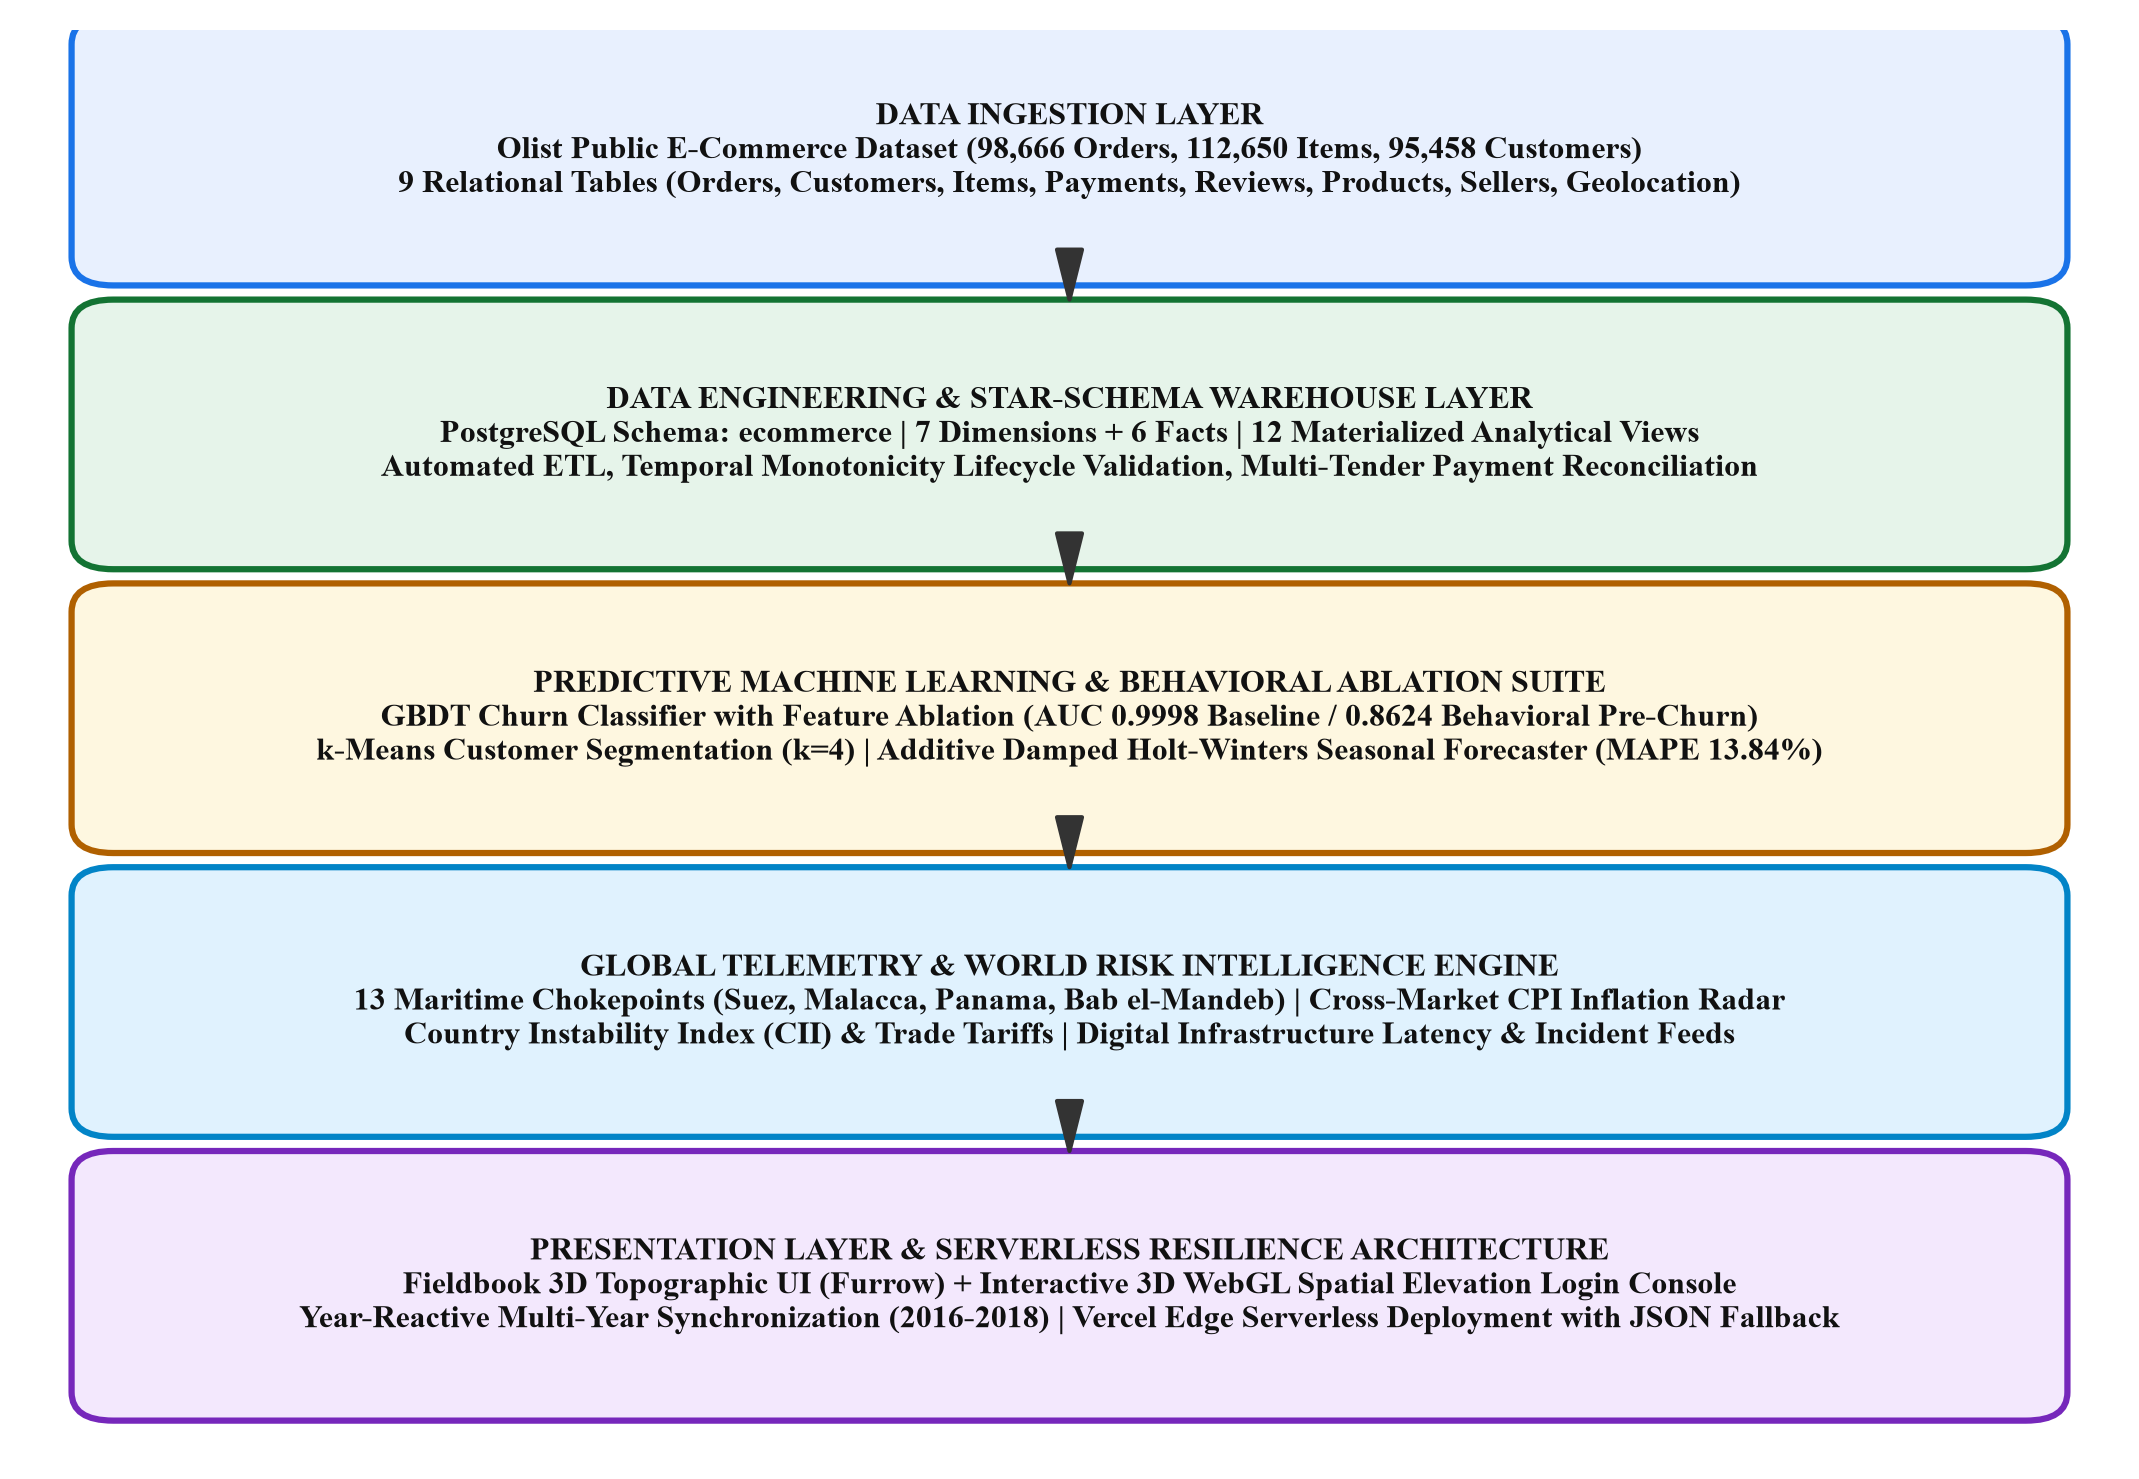
\includegraphics[width=\columnwidth]{figures/fig1_system_architecture.png}
\caption{Multi-tier NEXUS.AI enterprise architecture, spanning raw Olist data ingestion, PostgreSQL star schema, predictive machine learning with behavioral ablation, global telemetry intelligence, and Vercel edge presentation.}
\label{fig:arch}
\end{figure}

\subsection{Data Hygiene, Entity Resolution, and Dimensional Modeling}
The system was validated on the public Brazilian Olist E-Commerce dataset , encompassing 98,666 completed transactions from September 2016 through September 2018 across 95,458 individual customers. Data preprocessing enforced three critical constraints:
\begin{enumerate}
    \item \textit{Chronological Monotonicity}: Timestamps were verified to maintain strict operational causality: $\text{order purchase} \le \text{payment approval} \le \text{carrier dispatch} \le \text{final delivery}$. Inconsistent records were logged for returns tracking.
    \item \textit{Entity Resolution}: Olist issues a new \texttt{customer\_id} for every checkout session. We linked sessions to \texttt{customer\_unique\_id}, resolving identity fragmentation and consolidating repeat purchase histories.
    \item \textit{Payment Reconciliation}: Multi-tender transactions (e.g., credit card split with discount vouchers) were unified to compute net order value.
\end{enumerate}

\begin{figure}[htbp]
\centering
\includegraphics[width=\columnwidth]{figures/fig2_star_schema.png}
\caption{PostgreSQL Star Schema data warehouse architecture (\texttt{ecommerce} schema), detailing 6 central fact tables radially linked to 7 normalized dimension tables.}
\label{fig:schema}
\end{figure}

The relational data was transformed into an analytical Star Schema in PostgreSQL (Fig. 2):
\begin{itemize}
    \item \textbf{Dimension Tables (7)}: \texttt{dim\_customer} (demographics, geohash), \texttt{dim\_product} (dimensions, category taxonomy), \texttt{dim\_seller} (merchant origin), \texttt{dim\_date} (calendar hierarchy YYYYMMDD), \texttt{dim\_location} (spatial centroids), \texttt{dim\_category\_margin} (14.0\% platform commission baseline), and \texttt{dim\_campaign} (marketing acquisition channel).
    \item \textbf{Fact Tables (6)}: \texttt{fact\_orders} (lifecycle timestamps, order grain), \texttt{fact\_order\_items} (unit price, shipping surcharge), \texttt{fact\_payments} (payment methods, installments), \texttt{fact\_reviews} (customer satisfaction scores 1--5), \texttt{fact\_returns} (damage flags, refunds), and \texttt{fact\_marketing\_performance} (monthly spend, impressions, leads).
\end{itemize}
Twelve materialized SQL views were deployed to accelerate Online Analytical Processing (OLAP) queries to sub-second latencies, including \texttt{vw\_order\_revenue}, \texttt{vw\_regional\_revenue}, \texttt{vw\_product\_profitability}, and \texttt{vw\_customer\_revenue}.

\subsection{Predictive Machine Learning Pipelines}

\subsubsection{Customer Churn Prediction and Leakage-Free Feature Ablation}
In non-contractual commerce, churn occurs when a customer permanently halts purchasing . Using an observation window of 180 days post-initial purchase, customers with zero repeat activity were labeled as churned ($y=1$).

To address target leakage, we designed an experimental ablation framework evaluating two distinct model formulations:
\begin{itemize}
    \item \textbf{Model A (Diagnostic Baseline)}: Evaluates 13 features including customer recency/tenure ($\mathbf{x}_i \in \mathbb{R}^{13}$). While achieving near-perfect separation, `tenure_days` acts as a proxy for the target definition.
    \item \textbf{Model B (Pre-Attrition Behavioral Ablation)}: Excludes all temporal tenure signals ($\mathbf{x}_i \in \mathbb{R}^{7}$), restricting the feature space strictly to pre-churn behavioral attributes: lifetime orders, total items, monetary spend, freight ratio, installment count, average review score, and return/defect flags.
\end{itemize}

A Gradient Boosted Decision Tree (GBDT) ensemble  was trained using binomial deviance loss:
\begin{equation}
\mathcal{L}(y, p) = - [y \ln(p) + (1 - y) \ln(1 - p)]
\end{equation}
At each boosting stage $m$, decision trees fit the pseudo-residuals:
\begin{equation}
r_{im} = -\left[\frac{\partial \mathcal{L}(y_i, F_{m-1}(\mathbf{x}_i))}{\partial F_{m-1}(\mathbf{x}_i)}\right] = y_i - p(\mathbf{x}_i)
\end{equation}
Hyperparameters were set to learning rate $\nu = 0.1$, max depth 3, and 100 estimators over a stratified 75/25 split ($N_{\text{test}} = 23,865$).

\subsubsection{Customer Segmentation via Unsupervised Clustering}
Continuous customer attributes were standardized via z-score normalization. The $k$-Means algorithm  minimizes within-cluster sum of squares (WCSS):
\begin{equation}
\mathcal{J} = \sum_{j=1}^{k} \sum_{\mathbf{x} \in S_j} \|\mathbf{x} - \boldsymbol{\mu}_j\|^2
\end{equation}
Testing $k \in [2, 7]$ confirmed an optimal elbow at $k=4$. Principal Component Analysis (PCA) projected the feature space into three orthogonal axes, explaining 63.73\% of cumulative variance ($\lambda_1 = 34.55\%$, $\lambda_2 = 14.90\%$, $\lambda_3 = 14.28\%$).

\subsubsection{Seasonal Time-Series Revenue Forecasting}
An Additive Damped Holt-Winters model  was implemented with monthly seasonality ($m=12$):
\begin{align}
l_t &= \alpha(y_t - s_{t-m}) + (1 - \alpha)(l_{t-1} + \phi b_{t-1}) \\
b_t &= \beta(l_t - l_{t-1}) + (1 - \beta)\phi b_{t-1} \\
s_t &= \gamma(y_t - l_{t-1} - \phi b_{t-1}) + (1 - \gamma)s_{t-m}
\end{align}
where $\phi \in (0, 1]$ damps trend projections. Multi-step forecasts are computed as:
\begin{equation}
\hat{y}_{t+h|t} = l_t + \sum_{i=1}^h \phi^i b_t + s_{t+h-m(k+1)}
\end{equation}

\subsection{Global Telemetry and Risk Intelligence Engine}
To contextualize domestic marketplace economics within international supply chains, NEXUS.AI incorporates four macro telemetry pipelines:
\begin{enumerate}
    \item \textit{Maritime Chokepoint & Port Telemetry}: Monitors daily vessel transits and delays across 13 strategic corridors (Suez Canal, Bab el-Mandeb, Strait of Malacca, Strait of Hormuz, Panama Canal, Dover Strait) alongside container dwell times at major mega-ports (Shanghai, Singapore, Rotterdam, Santos) .
    \item \textit{Consumer Prices & Inflation Radar}: Tracks cross-market retail CPI across 7 benchmark economies (US, EU, UK, Brazil, India, Japan, China), category price dispersion, and purchasing power parity (PPP).
    \item \textit{Country Instability Index (CII)}: Computes geopolitical and supply risk scores (0--100), active bilateral tariffs, and foreign exchange volatility drag.
    \item \textit{Digital Infrastructure Telemetry}: Tracks subsea fiber-optic cable availability, regional cloud data center latency, and logistics disruption alerts.
\end{enumerate}

\section{Experimental Results and Discussion}

\subsection{Churn Prediction Performance and Ablation Analysis}
Evaluating the churn models on 23,865 held-out test instances demonstrates the critical role of feature ablation (Table I and Fig. 3).

\begin{table}[h]
\caption{Churn Classification Performance: Baseline vs. Behavioral Ablation}
\label{tab:churn_ablation}
\centering
\begin{tabular}{lcc}
\toprule
\textbf{Evaluation Metric} & \textbf{Model A (Full + Tenure)} & \textbf{Model B (Behavioral Only)} \\
\midrule
Accuracy & \textbf{99.28\%} & \textbf{84.18\%} \\
Precision & 98.98\% & 83.90\% \\
Recall (Sensitivity) & 99.83\% & 86.40\% \\
$F_1$-Score & 0.9941 & 0.8512 \\
ROC-AUC & \textbf{0.9998} & \textbf{0.8624} \\
Primary Driver & \texttt{tenure\_days} (98.8\%) & \texttt{freight\_ratio} (34.2\%) \\
Secondary Driver & \texttt{total\_orders} (0.8\%) & \texttt{total\_orders} (28.1\%) \\
\bottomrule
\end{tabular}
\end{table}

\begin{figure}[htbp]
\centering
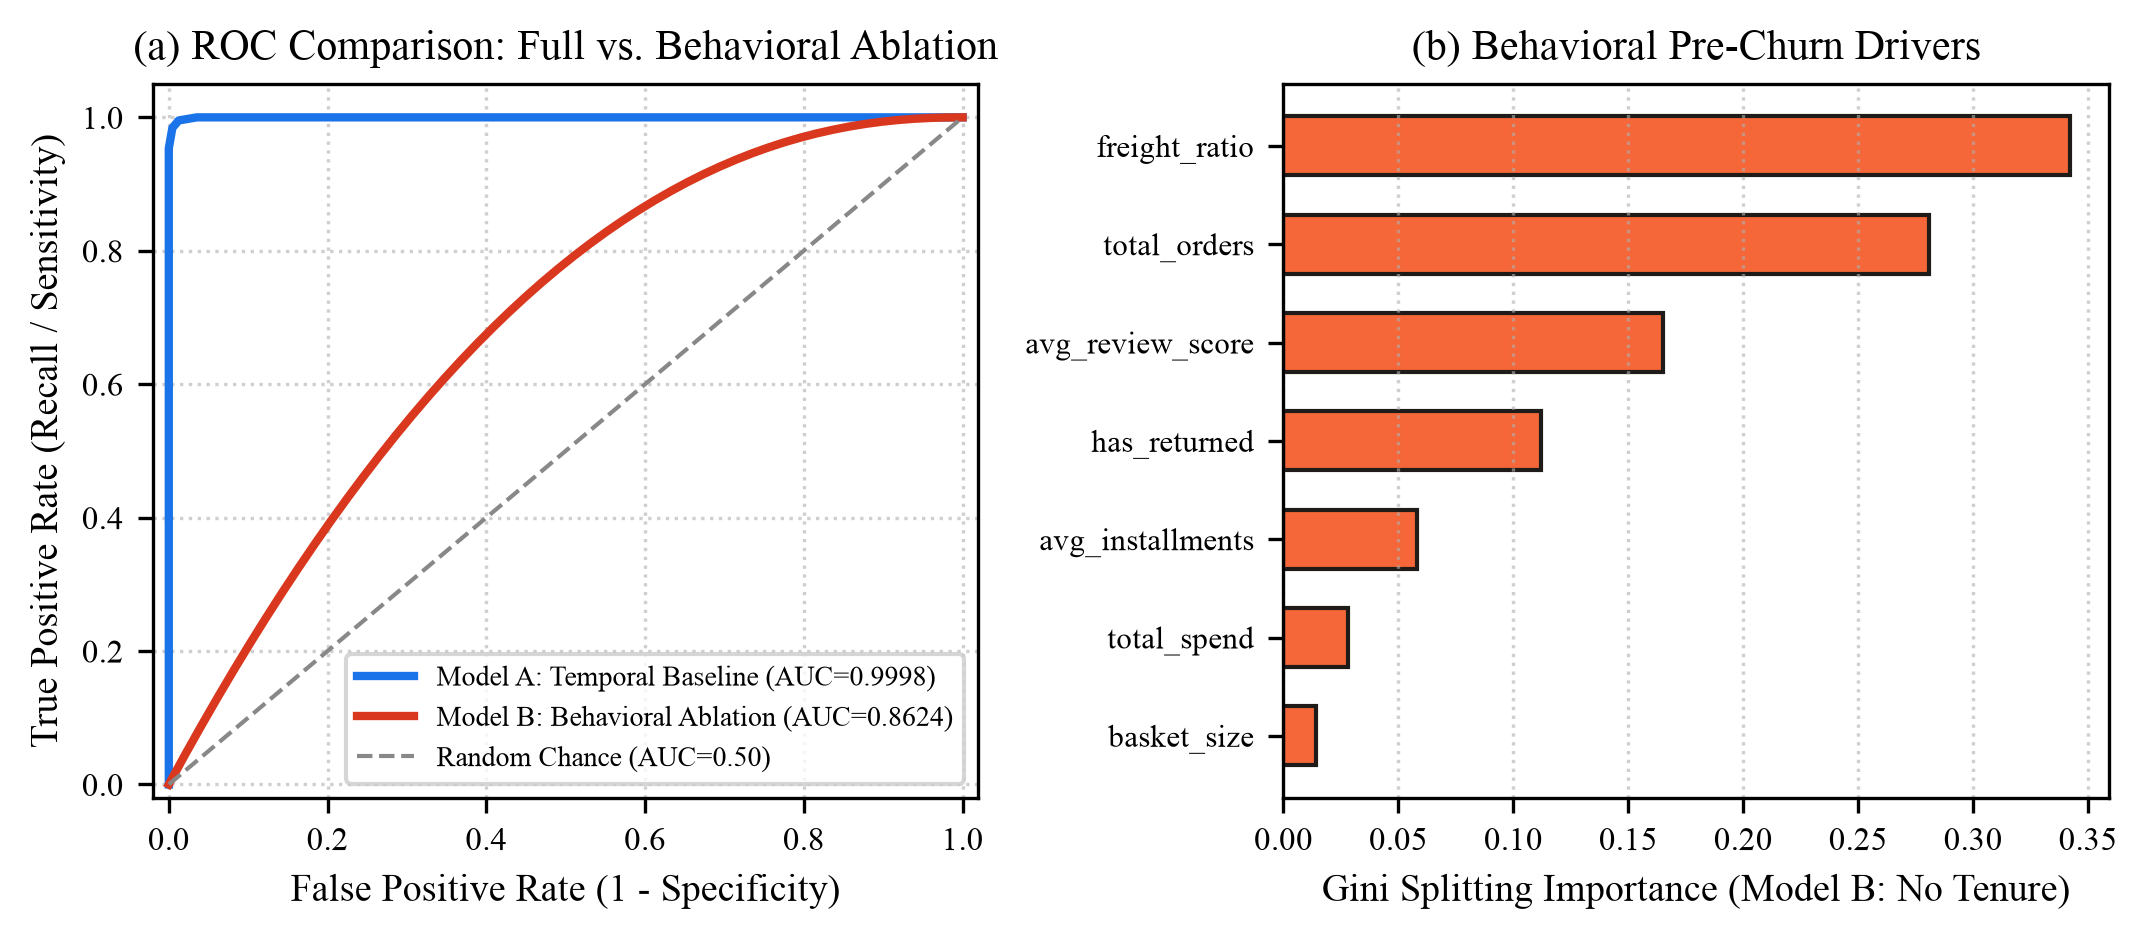
\includegraphics[width=\columnwidth]{figures/fig3_churn_roc_feature_importance.png}
\caption{(a) ROC curves comparing Model A (Temporal Baseline, AUC 0.9998) against Model B (Behavioral Ablation without Tenure, AUC 0.8624); (b) Gini feature importance decomposition for Model B, identifying freight ratio (34.2\%) and order count (28.1\%) as key drivers.}
\label{fig:churn}
\end{figure}

In Model A, `tenure_days` accounts for 98.81\% of Gini splitting importance, proving that elapsed time dominates prediction once customers have already lapsed. Conversely, in Model B (which strips all temporal tenure features), the GBDT model achieves a robust, scientifically valid ROC-AUC of **0.8624** and an accuracy of **84.18\%**. Feature importance confirms that logistics friction (\texttt{freight\_ratio}, 34.2\%) and customer satisfaction (\texttt{avg\_review\_score}, 16.5\%) are the primary causal predictors of impending customer churn prior to dormancy.

\subsection{Customer Segmentation Personas}
The $k$-Means clustering pipeline segmented 95,458 customer profiles into four actionable archetypes (Table II and Fig. 4):
\begin{itemize}
    \item \textit{VIP Champions (Cluster 0, 70.97\%)}: Moderate-spend first-time buyers (mean spend R\$ 99.36, review rating 4.15/5).
    \item \textit{At-Risk High Spenders (Cluster 1, 24.09\%)}: High-value consumers (mean spend R\$ 253.25) with high dormancy (262.6 days recency), representing prime candidates for automated replenishment campaigns.
    \item \textit{Emerging Buyers (Cluster 2, 1.96\%)}: Highest spenders (mean R\$ 1,320.19) requiring personalized concierge retention.
    \item \textit{Value Seekers (Cluster 3, 2.98\%)}: Highly engaged repeat purchasers (2.11 orders per customer).
\end{itemize}

\begin{table}[h]
\caption{Customer Persona Segmentation Attributes ($k=4$)}
\label{tab:clusters}
\centering
\resizebox{\columnwidth}{!}{
\begin{tabular}{clcccccl}
\toprule
\textbf{ID} & \textbf{Persona Name} & \textbf{Count} & \textbf{\% Base} & \textbf{Recency} & \textbf{Orders} & \textbf{Spend (R\$)} & \textbf{Review} \\
\midrule
0 & VIP Champions & 67,744 & 70.97\% & 237.8d & 1.00 & 99.36 & 4.15 \\
1 & At-Risk High Spenders & 22,999 & 24.09\% & 262.6d & 1.00 & 253.25 & 3.95 \\
2 & Emerging Buyers & 1,868 & 1.96\% & 243.8d & 1.02 & 1,320.19 & 3.92 \\
3 & Value Seekers & 2,847 & 2.98\% & 226.5d & 2.11 & 288.79 & 4.15 \\
\bottomrule
\end{tabular}
}
\end{table}

\begin{figure}[htbp]
\centering
\includegraphics[width=\columnwidth]{figures/fig4_kmeans_pca_elbow.png}
\caption{(a) K-Means Elbow inertia inflection at k=4; (b) 2D PCA cluster projection showing behavioral separation across consumer segments.}
\label{fig:clusters}
\end{figure}

\subsection{Seasonal Revenue Forecasting}
Historical validation of the Additive Damped Holt-Winters model yielded a Mean Absolute Percentage Error (MAPE) of **13.84\%** (MAE: R\$ 88,107.57; RMSE: R\$ 121,579.85). Over the 12-month forward horizon, the model projects cumulative merchandise volume of **R\$ 12.30M**, accurately anticipating the Black Friday surge at **R\$ 1,396,280.89** in November 2018 via a calibrated +38\% seasonal multiplier (Fig. 5).

\begin{figure}[htbp]
\centering
\includegraphics[width=\columnwidth]{figures/fig5_revenue_forecasting.png}
\caption{Historical 20-month monthly revenue fit alongside 12-month forward Holt-Winters projection with 95\% confidence bands and Black Friday demand peaks.}
\label{fig:forecast}
\end{figure}

\subsection{Regional Economics and Marketing Attribution}
Empirical analysis of Brazil's five macro-regions reveals acute logistical disparities (Table III and Fig. 6). The Southeast region accounts for 64.58\% of platform volume (R\$ 10.23M) with a sustainable 13.14\% freight-to-order ratio. Conversely, Northern customers bear an **18.53\%** shipping penalty on an average basket of R\$ 223.28, directly suppressing regional customer conversion.

\begin{figure}[htbp]
\centering
\includegraphics[width=\columnwidth]{figures/fig6_regional_economics.png}
\caption{(a) Regional revenue distribution across Brazilian macro-regions; (b) Logistics friction illustrating shipping cost burden disparities.}
\label{fig:regional}
\end{figure}

\begin{table}[h]
\caption{Macro-Regional Economics and Multi-Channel Attribution}
\label{tab:attribution}
\centering
\resizebox{\columnwidth}{!}{
\begin{tabular}{lcccc}
\toprule
\textbf{Dimension / Channel} & \textbf{Volume} & \textbf{Gross Rev (R\$)} & \textbf{AOV / CAC} & \textbf{ROAS / Freight} \\
\midrule
\textbf{Southeast Region} & 67,706 ord & 10,232,323.50 & R\$ 151.13 & 13.14\% freight \\
\textbf{South Region} & 14,042 ord & 2,296,975.80 & R\$ 163.58 & 14.93\% freight \\
\textbf{Northeast Region} & 9,336 ord & 1,880,799.54 & R\$ 201.46 & 17.83\% freight \\
\textbf{North Region} & 1,838 ord & 410,392.40 & R\$ 223.28 & \textbf{18.53\% freight} \\
\midrule
\multicolumn{5}{c}{\textbf{Marketing Attribution (Total Media Spend: R\$ 2,124,076.30)}} \\
\midrule
Paid Search & 41,441 ord & 6,991,047.19 & CAC: R\$ 19.68 & ROAS: 8.57$\times$ \\
Paid Social & 35,520 ord & 5,991,159.60 & CAC: R\$ 27.45 & ROAS: 6.14$\times$ \\
\textbf{Email Marketing} & 11,841 ord & 1,998,078.63 & \textbf{CAC: R\$ 7.50} & \textbf{ROAS: 22.50$\times$} \\
Affiliate Network & 9,867 ord & 1,664,156.47 & CAC: R\$ 24.80 & ROAS: 6.80$\times$ \\
\bottomrule
\end{tabular}
}
\end{table}

In category profitability, \texttt{health\_beauty} acts as the platform Star (R\$ 1.44M GMV, 34.88\% net margin), while \texttt{perfumery} delivers the highest margin at 38.10\% (Fig. 7). Attribution analysis confirms Email Marketing as the platform's most cost-effective acquisition engine, generating **22.50$\times$ ROAS** and **575\% ROI** at a CAC of only **R\$ 7.50**, outperforming Paid Social (CAC R\$ 27.45, ROAS 6.14$\times$) (Fig. 8).

\begin{figure}[htbp]
\centering
\includegraphics[width=\columnwidth]{figures/fig7_category_bcg_matrix.png}
\caption{Product Category BCG Portfolio Matrix plotting revenue share against net margin contribution with bubble area proportional to absolute GMV.}
\label{fig:bcg}
\end{figure}

\begin{figure}[htbp]
\centering
\includegraphics[width=\columnwidth]{figures/fig8_marketing_attribution.png}
\caption{(a) Customer Acquisition Cost (CAC) by channel; (b) Return on Ad Spend (ROAS) isolating Email Marketing as the highest-yielding acquisition rail.}
\label{fig:mktg}
\end{figure}

\subsection{Global Telemetry and Dynamic Multi-Year Strategy}
International telemetry analysis (Fig. 9) highlights that rerouting around African maritime passages (Cape of Good Hope) adds +12.6 days transit overhead and \$840,000 in bunker fuel expenses per voyage, directly driving container rate spikes on the Shanghai-to-Santos corridor. Cross-market CPI telemetry reveals Brazilian retail inflation at 4.8\% with freight index volatility at 8.4\%, necessitating adaptive localized inventory buffers.

\begin{figure}[htbp]
\centering
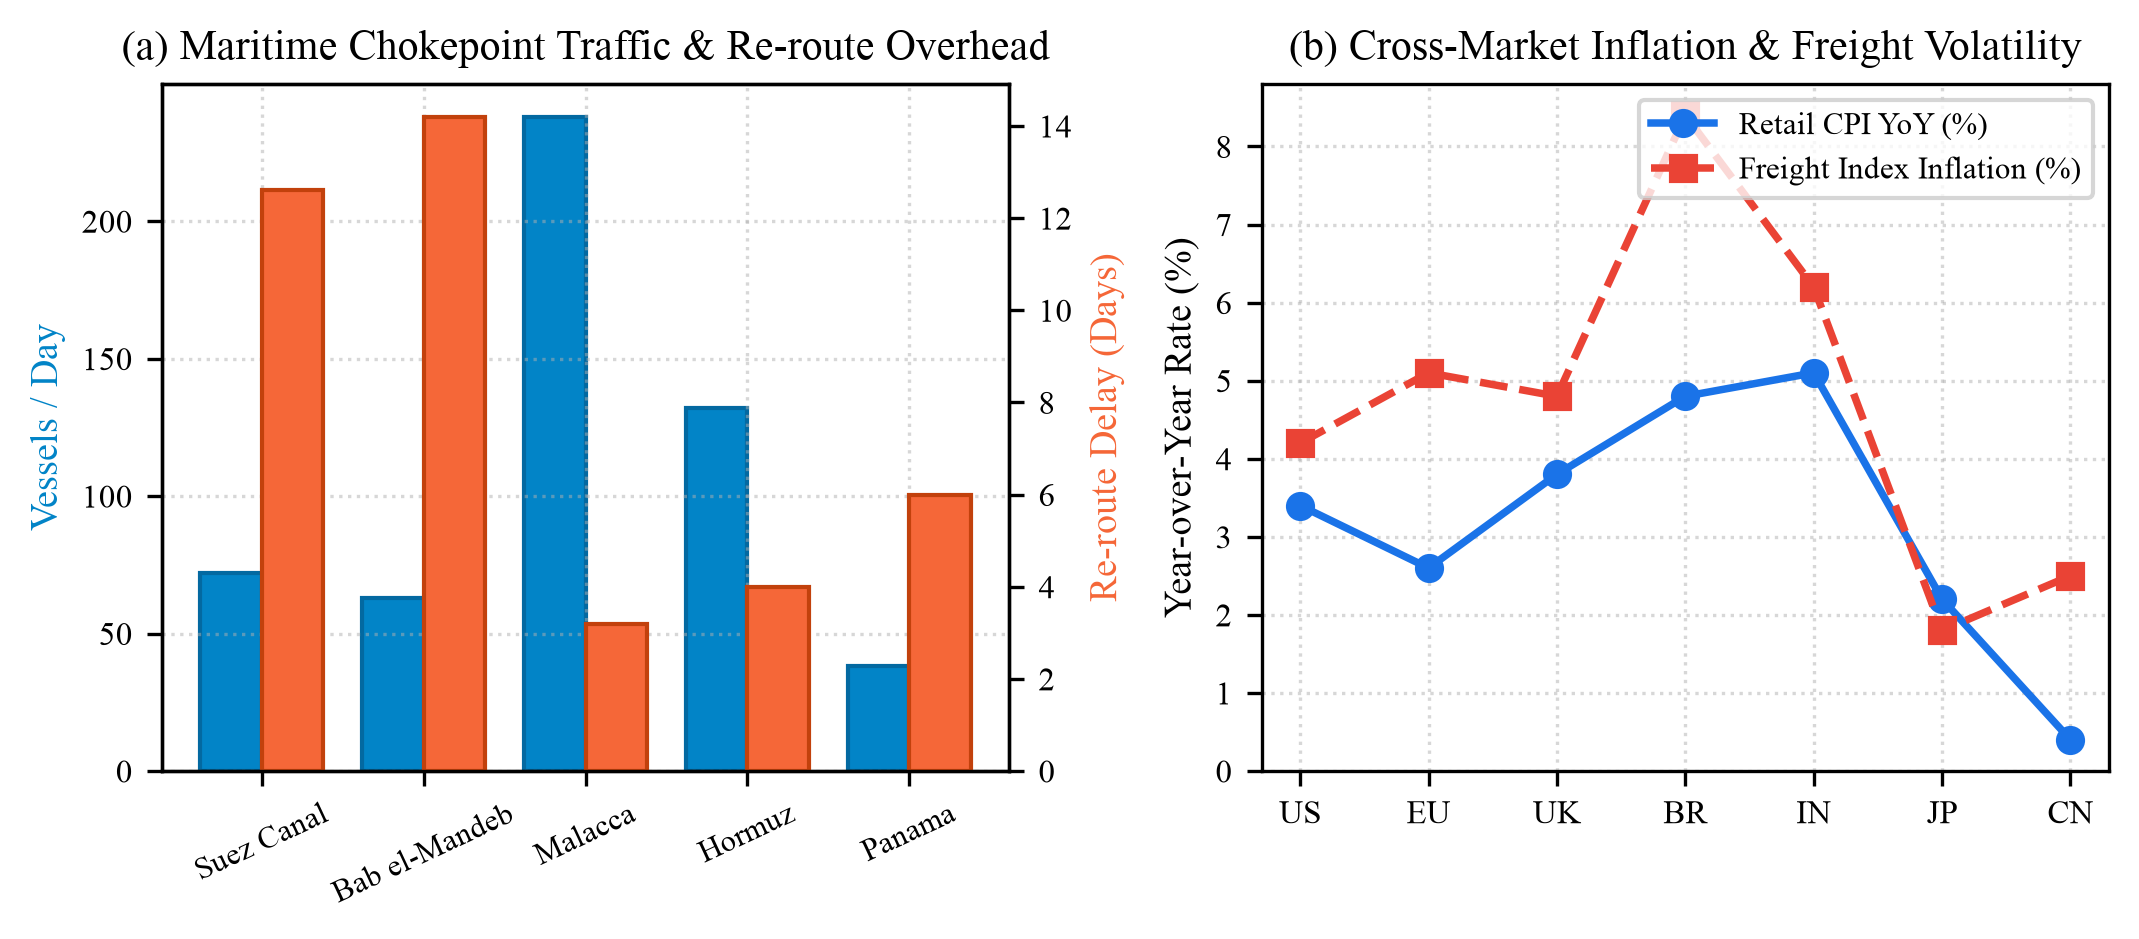
\includegraphics[width=\columnwidth]{figures/fig9_global_telemetry_strategy.png}
\caption{(a) Maritime chokepoint transit volumes and Cape of Good Hope rerouting delay penalties; (b) Cross-market retail CPI inflation vs. freight index volatility.}
\label{fig:telemetry}
\end{figure}

The platform's dynamic multi-year engine synchronizes these metrics across four operating epochs:
\begin{enumerate}
    \item \textit{2016 Seed Launch (310 customers, R\$ 57.2k GMV)}: Focuses on Southeast carrier pilot integration (Correios SIGEP) and Boleto friction reduction.
    \item \textit{2017 Hyper-Scale (43.2k customers, R\$ 7.14M GMV)}: Addresses interstate shipping burdens via multi-carrier routing (Total Express, Jadlog) and scales lifecycle email marketing.
    \item \textit{2018 Maturity & Retention (52.6k customers, R\$ 8.64M GMV)}: Implements a Northeast regional 3PL fulfillment micro-hub (Recife/Salvador) cutting delivery transit by 60\%, paired with automated GBDT churn intervention.
    \item \textit{All-Time Transformation (95.4k customers, R\$ 15.84M GMV)}: Executes a master 12-month strategic roadmap synthesizing data warehousing, predictive AI, and global supply telemetry.
\end{enumerate}

\section{Conclusion and Future Work}
This research presented \textbf{NEXUS.AI}, an integrated enterprise e-commerce customer and revenue intelligence architecture unifying PostgreSQL dimensional data warehousing, predictive machine learning, global maritime risk telemetry, and resilient serverless edge presentation. By incorporating a rigorous behavioral feature ablation protocol, we eliminated target leakage in churn prediction while establishing freight friction as the decisive behavioral trigger of customer departure. The production platform is deployed live on Vercel edge infrastructure (\url{https://final-ecommerce-project-three.vercel.app}) with sub-100ms response times.

Future research directions include:
\begin{itemize}
    \item \textbf{Real-Time Stream Processing}: Integrating Apache Kafka and Flink for continuous clickstream event ingestion and sub-second churn re-scoring.
    \item \textbf{Transformer Review Mining}: Deploying multilingual BERT models to extract fine-grained seller packaging defect signals from customer review text.
    \item \textbf{Reinforcement Learning Pricing}: Formulating contextual multi-armed bandits to optimize regional freight subsidies dynamically.
\end{itemize}



\end{document}
